\suppnote{Joint spectra and coherent response}{note:spectral}

\paragraph{Joint temporal--spatial spectrum.} For raw field $v_{d,j}$ on a TRAIN-date block of length $N$, a unitary one-sided discrete Fourier transform gives
\begin{equation}
\begin{aligned}
 Z_{d,m}&=N^{-1/2}\sum_{j=0}^{N-1}v_{d,j}e^{-2\pi imj/N},\qquad f_m=m/N,\\
 P_m&=w_m\langle\norm{Z_{d,m}}^2\rangle_d,\qquad
 J_{m,k}=\frac{P_m}{\sum_lP_l}\frac{s_{m,k}^2}{\sum_a s_{m,a}^2}.
\end{aligned}
\label{eq:supp-joint-spectrum}
\end{equation}
Here $s_{m,k}$ are singular values of the date-by-space coefficient matrix, $w_0=w_{N/2}=1$, and interior weights are two. The transform retains $m=0$, so the spectra include each date's phase mean. Porto and San Francisco use $N=24$; Chengdu uses $N=18$ for 06--23\,h without night imputation or zero filling. San Francisco averages $P_m$ and within-frequency mode shares separately across TRAIN folds before multiplication. Normalization uses the full weighted spectrum before the eight-mode display cut in Figure~\ref{fig:supp-1}. Spatial modes are frequency-specific singular modes, not geographical Fourier wavelengths.

Chengdu has ten single-sided bins $m=0,\ldots,9$ at $m/18$ cycles per observed hour. The periodic extension joins the ends of the observed block; it does not infer the unobserved night. A 24-hour sinusoid is off this grid, so the first nonzero bin is not identified as the once-daily harmonic. Zero padding to 24 samples would change the frequency grid and redistribute shares, not establish zero night-time flow.

\begin{figure}[!htbp]
\centering
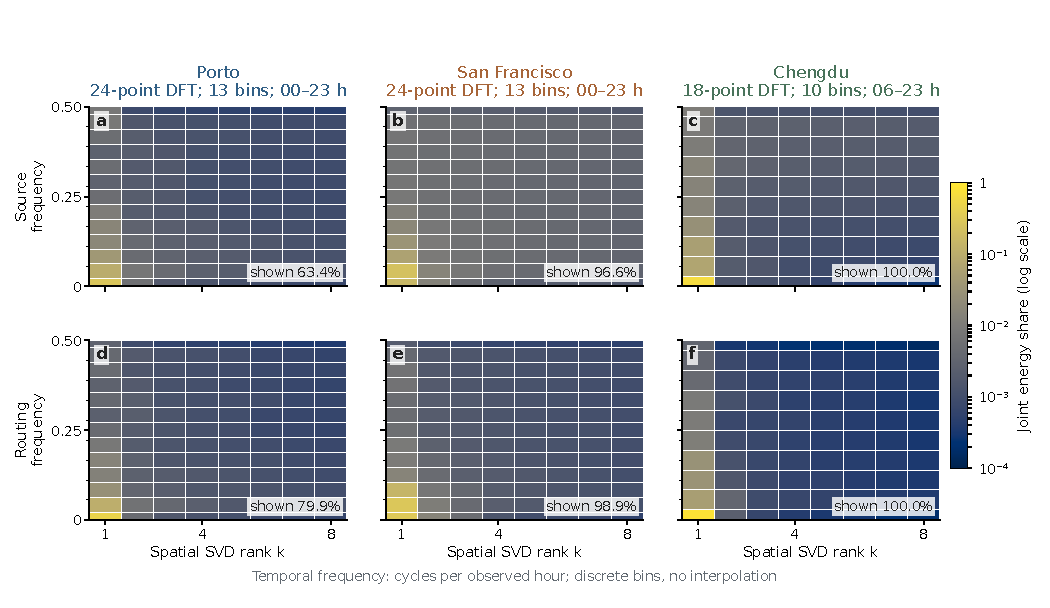
\includegraphics[width=\textwidth]{figures_supp/figS01_joint_spectrum_2d.pdf}
\caption{\textbf{Three-city two-dimensional joint spectra.} Joint energy share over temporal frequency and frequency-specific spatial mode rank for source and full-face routing fields in Porto, San Francisco and Chengdu. The eight-mode display cut is applied after full-spectrum normalization. Porto and San Francisco use 24-point DFTs; Chengdu uses an 18-point observed-block DFT with no night imputation. San Francisco averages frequency energies and within-frequency mode shares separately across TRAIN folds. Spatial rank is not geographical wavelength.}
\label{fig:supp-1}
\end{figure}

\begin{figure}[!htbp]
\centering
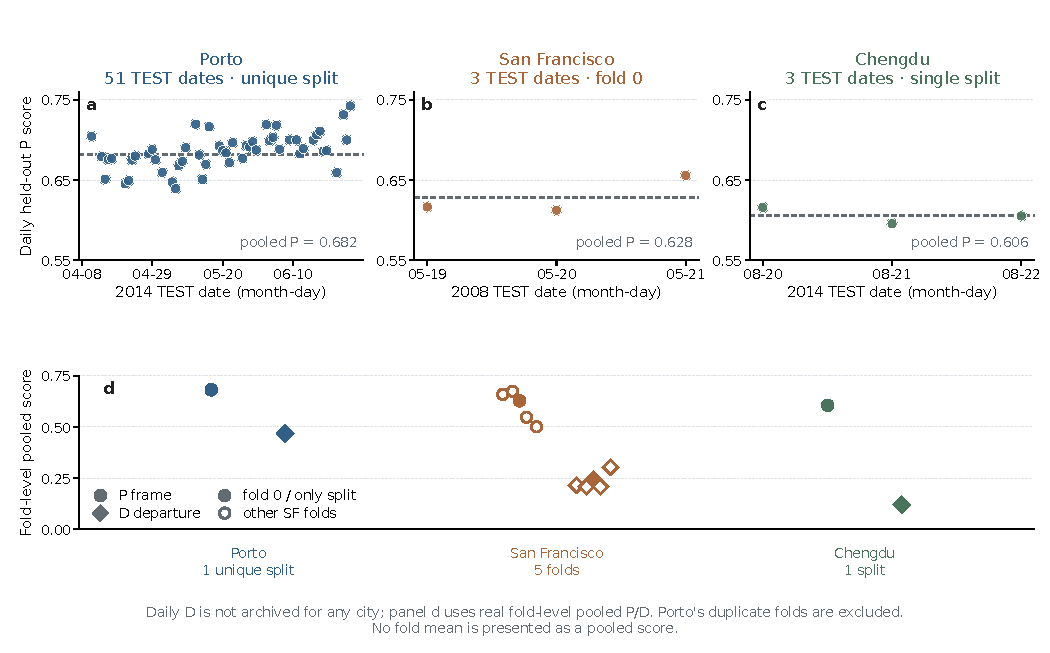
\includegraphics[width=0.95\textwidth]{figures_supp/figS02_heldout_daily_scores.pdf}
\caption{\textbf{Three-city held-out daily P/D scores.} Date-specific P and D values for Porto, San Francisco and Chengdu under the frozen splits in Table~\ref{tab:observation-regimes}. San Francisco retains its five-fold structure; Chengdu has three TEST dates in the continuous-observation protocol. Daily values complement the pooled scores in Table~\ref{tab:crosscity}; their spread is not a paired-date confidence interval.}
\label{fig:supp-2}
\end{figure}

\paragraph{Coherent TRAIN/TEST response.} The frozen P-selected operator is applied without refitting a frequency response. Each date is transformed with the same unitary DFT support as the descriptive spectrum: 24 points in Porto and San Francisco and 18 points in Chengdu. Let $a_m^{(\mathcal S)}$ and $b_m^{(\mathcal S)}$ be observed and predicted routing coefficients averaged over dates in split $\mathcal S\in\{\mathrm{TRAIN},\mathrm{TEST}\}$. For each split and single-sided bin $m$,
\begin{equation}
 \gamma_m^{(\mathcal S)}=\frac{|a_m^{(\mathcal S)*}b_m^{(\mathcal S)}|}{\norm{a_m^{(\mathcal S)}}\norm{b_m^{(\mathcal S)}}},
 \qquad
 \rho_m^{(\mathcal S)}=\frac{\norm{b_m^{(\mathcal S)}}}{\norm{a_m^{(\mathcal S)}}} .
 \label{eq:supp-coherent-response}
\end{equation}
The absolute inner product makes $\gamma_m$ insensitive to a common phase rotation. TRAIN values describe the fit sample; TEST values are held-out. San Francisco summaries are fold means and ranges. These coherent averages complement, rather than replace, observation-level P/D scores. Chengdu evaluates all ten bins $m=0,\ldots,9$, exactly as in its joint spectrum. Figure~\ref{fig:supp-3} displays both splits without treating the TRAIN comparison as independent validation.

\begin{figure}[!htbp]
\centering
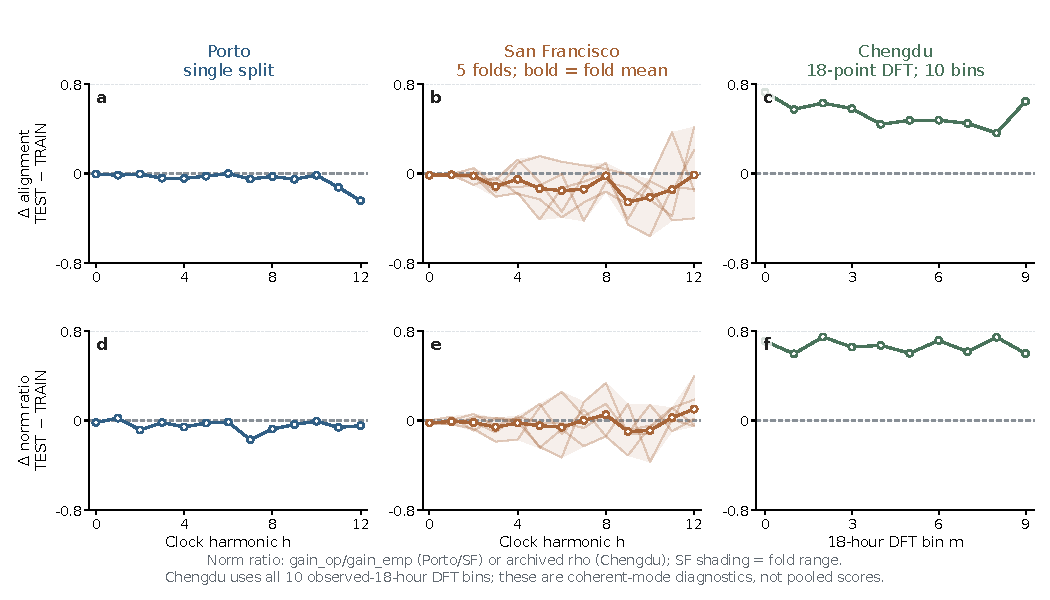
\includegraphics[width=\textwidth]{figures_supp/figS03_coherent_response_train_test.pdf}
\caption{\textbf{Three-city coherent response on TRAIN and TEST.} Direction alignment $\gamma_m$ and predicted-to-observed norm ratio $\rho_m$ for Porto, San Francisco and Chengdu under the frozen P-selected operator. TRAIN values describe the fit sample; TEST values are held-out. San Francisco shows fold means and ranges. Each date uses the same unitary DFT support as the descriptive spectrum; Chengdu evaluates all ten single-sided bins of its 18-point transform. Alignment is insensitive to a common phase rotation.}
\label{fig:supp-3}
\end{figure}
